
\section{Introduction \DDC}
\label{chap2:intro}
%\textcolor{orange}{
%In the past few years, Body Biasing Injection has been getting more and more attention.
%Indeed, it is a low-cost method which requires a low bill of material, roughly compsoed of:
%\begin{itemize}
%    \item A voltage pulse generator
%    \item A metallic probe
%    \item A target IC
%    \item Cables to interconnect equipment
%\end{itemize}
%The most expensive piece of equipment is definitely the voltage pulse generator.
%However, there are low-cost solutions like the NewAE ChipSHOUTER for example, which can easily replace high voltage high precision generator in some use cases.}
%Nonetheless, during this work, the generator used is the AVTECH AVRK-4-B, which a high speed, precise, voltage pulse generator.
%It allows generating positive or negative pulses up to 750 V of amplitude with a 4 ns rise or fall time, with pulse widths ranging from 6 ns to 20 ns.
%It allowed us to finely tune each setting in order to perform reproducible experiments.
%
%Another very important piece of equipment used for BBI is the probe.
%It simply consists in a metallic tip soldered to an SMA connector.
%However,

\subsection{Platform equipment \DDC}
\label{chap2:intro:platEquip}
This section is dedicated in presenting the different piece of equipment which allowed us to perform this work.
The hardware platform, as well as the different software used are introduced.

\subsection{The hardware \DDC}
\label{chap2:intro:platEquip:hardware}

%\begin{figure}[H]
%    \centering
%    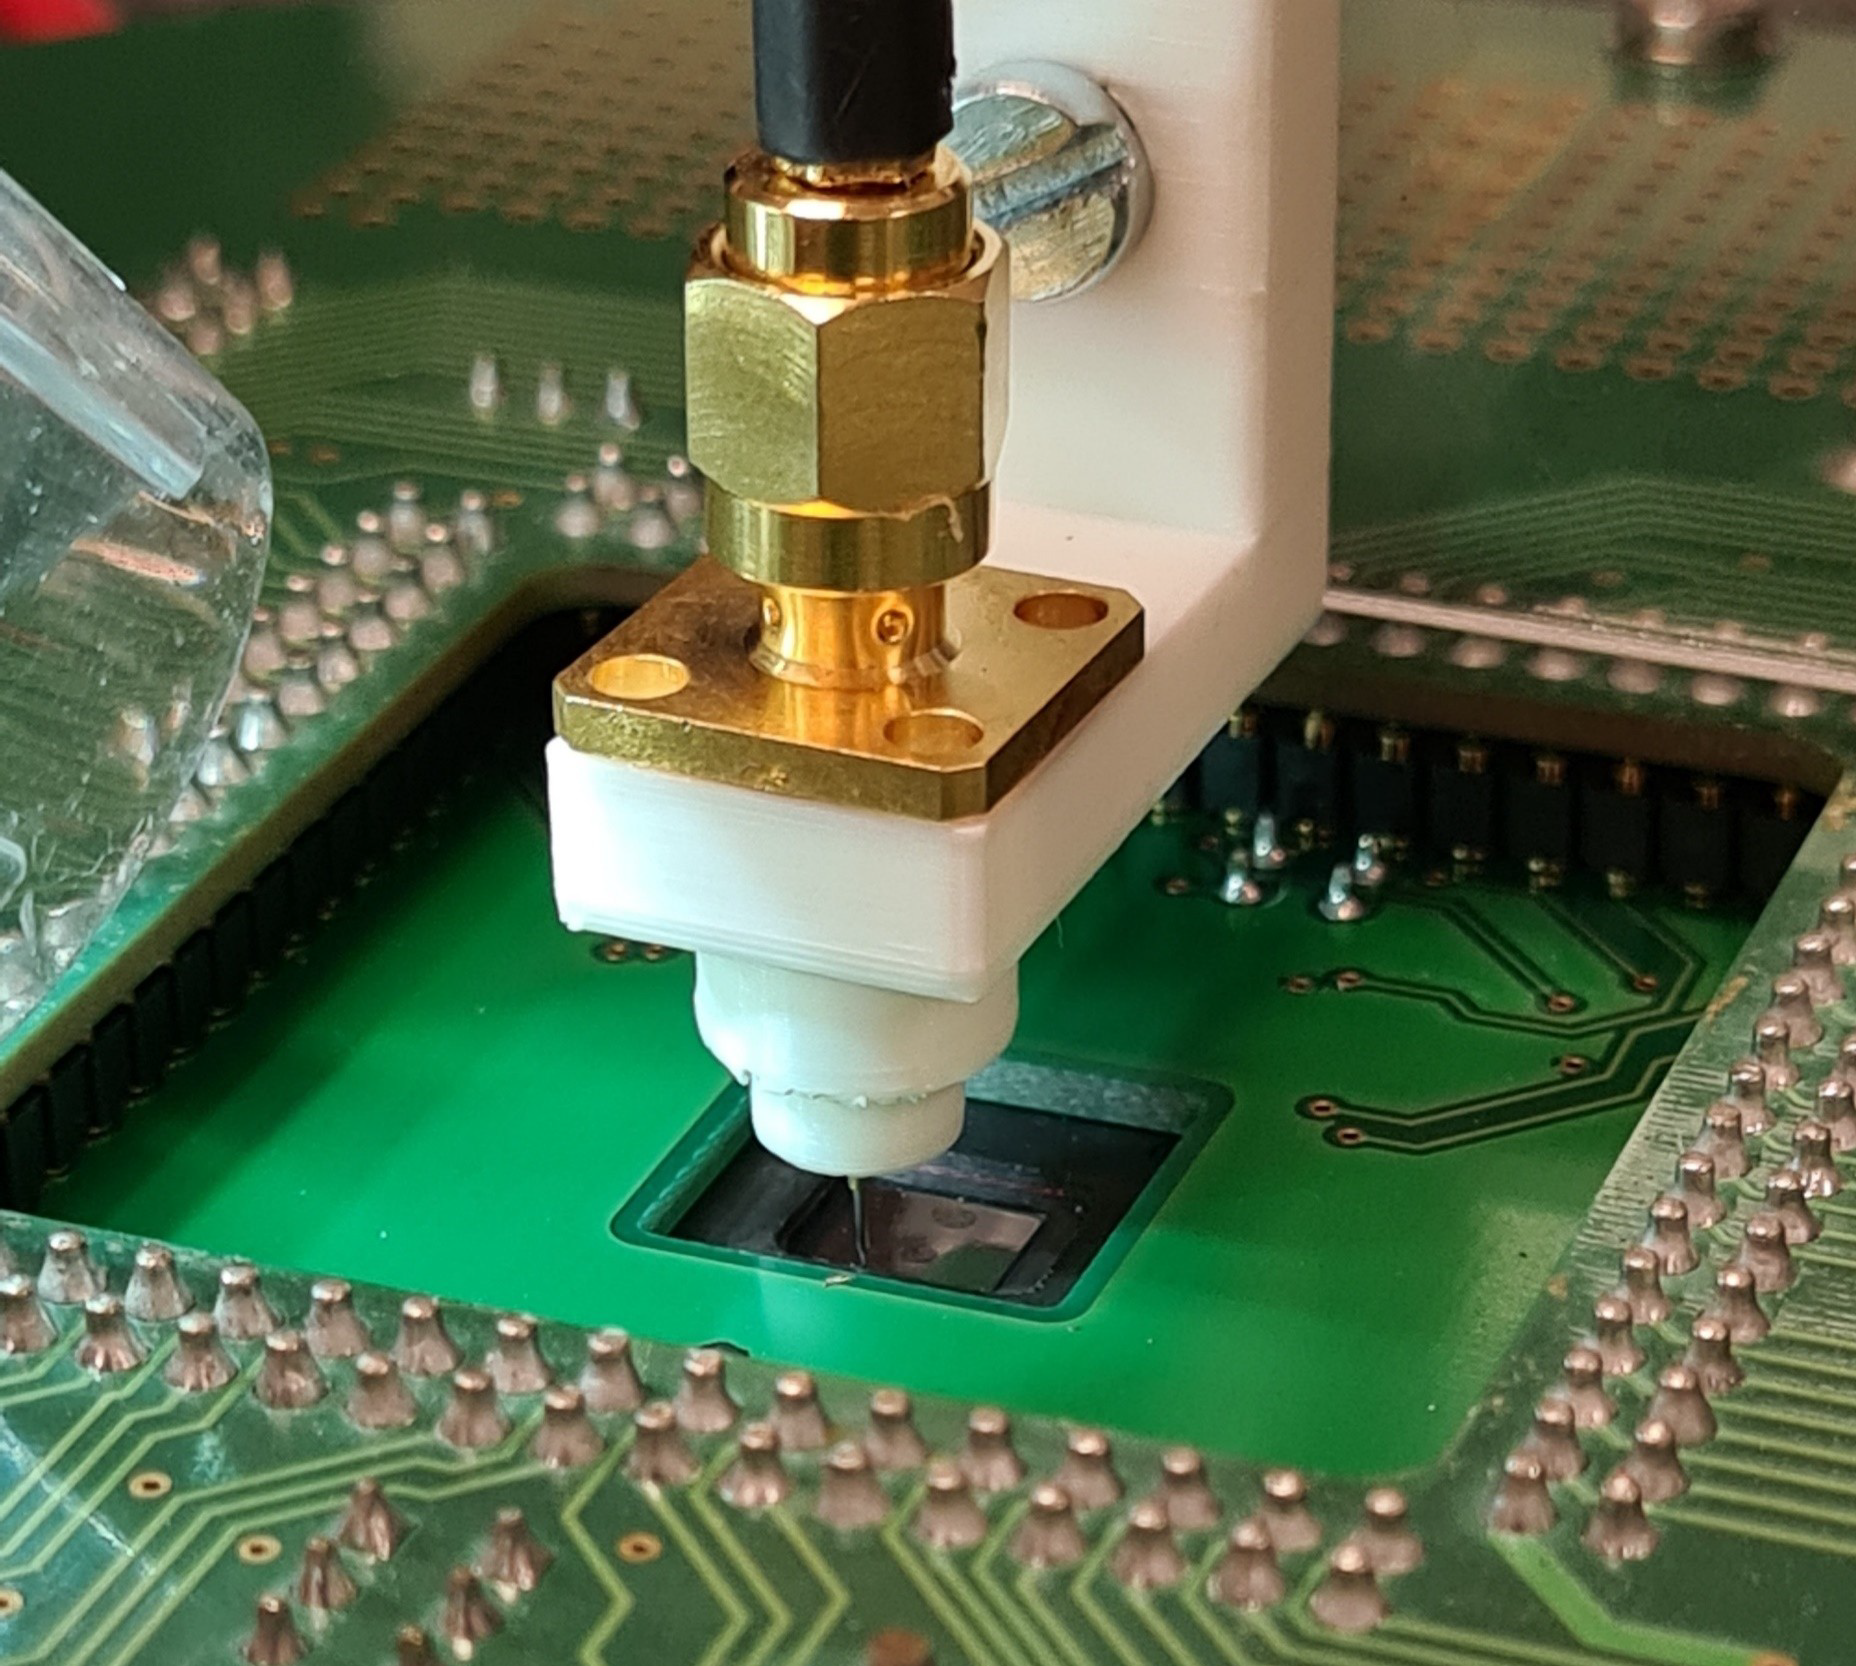
\includegraphics[width=16cm]{2_goodPractices/figures/sondeBBI_loin_raw.png}
%    \caption{BBI metallic probe in mechanical contact with IC target}
%    \label{fig:sondeBBI}
%\end{figure}
%
%\begin{figure}[H]
%    \centering
%    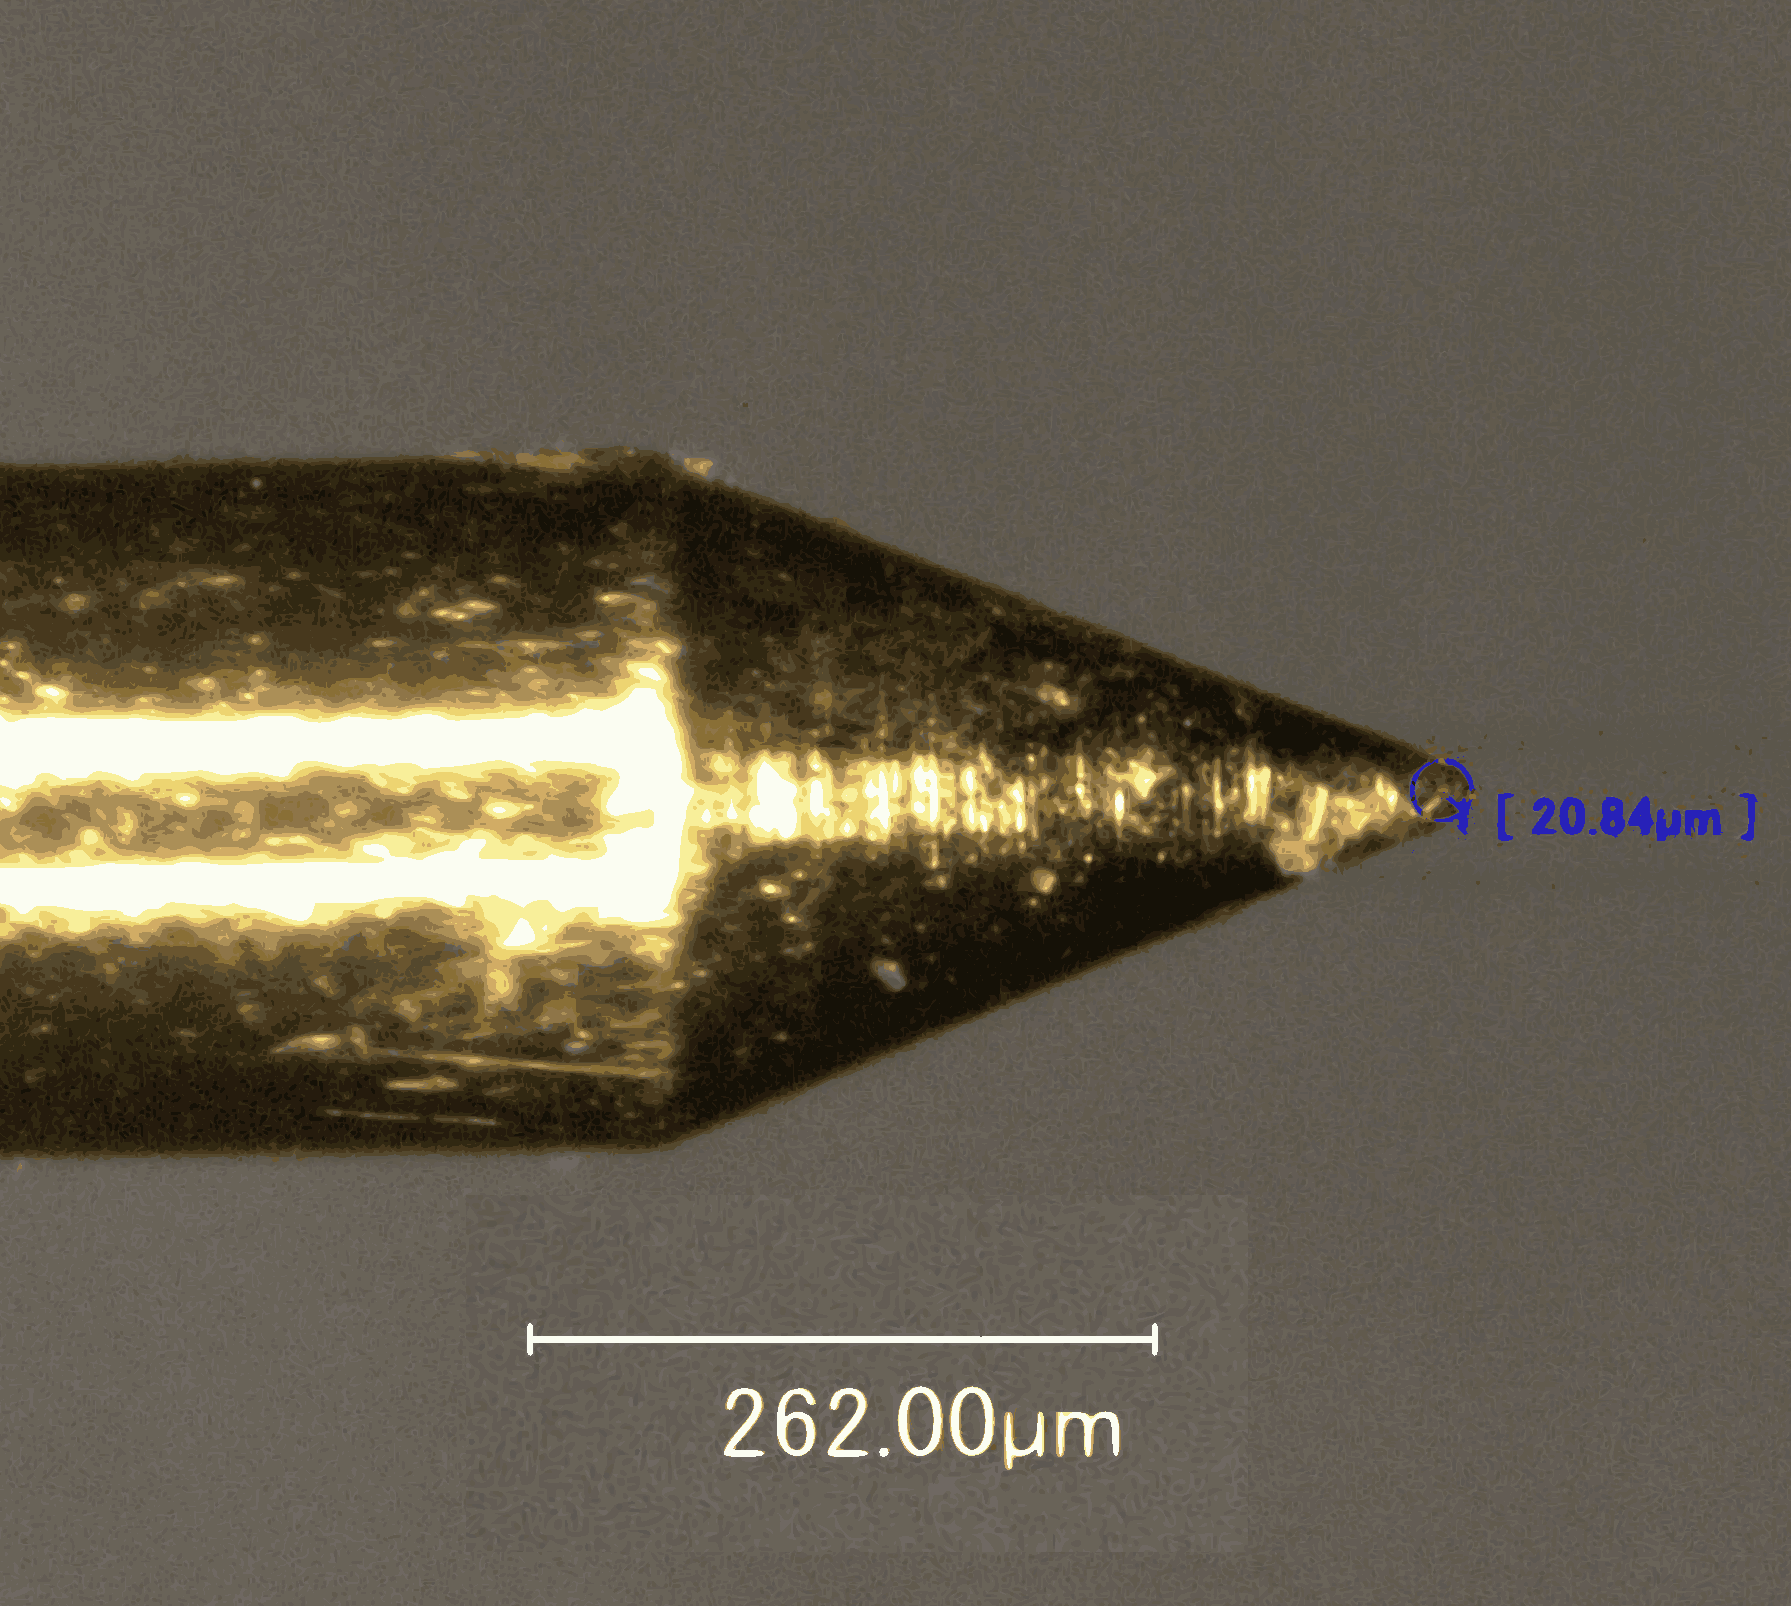
\includegraphics[width=16cm]{2_goodPractices/figures/pointeBBI.pdf}
%    \caption{BBI metallic probe measurement closer look}
%    \label{fig:pointeBBI}
%\end{figure}

\begin{figure}[ht!]
    \centering
    \begin{subfigure}[t]{7.0cm}
        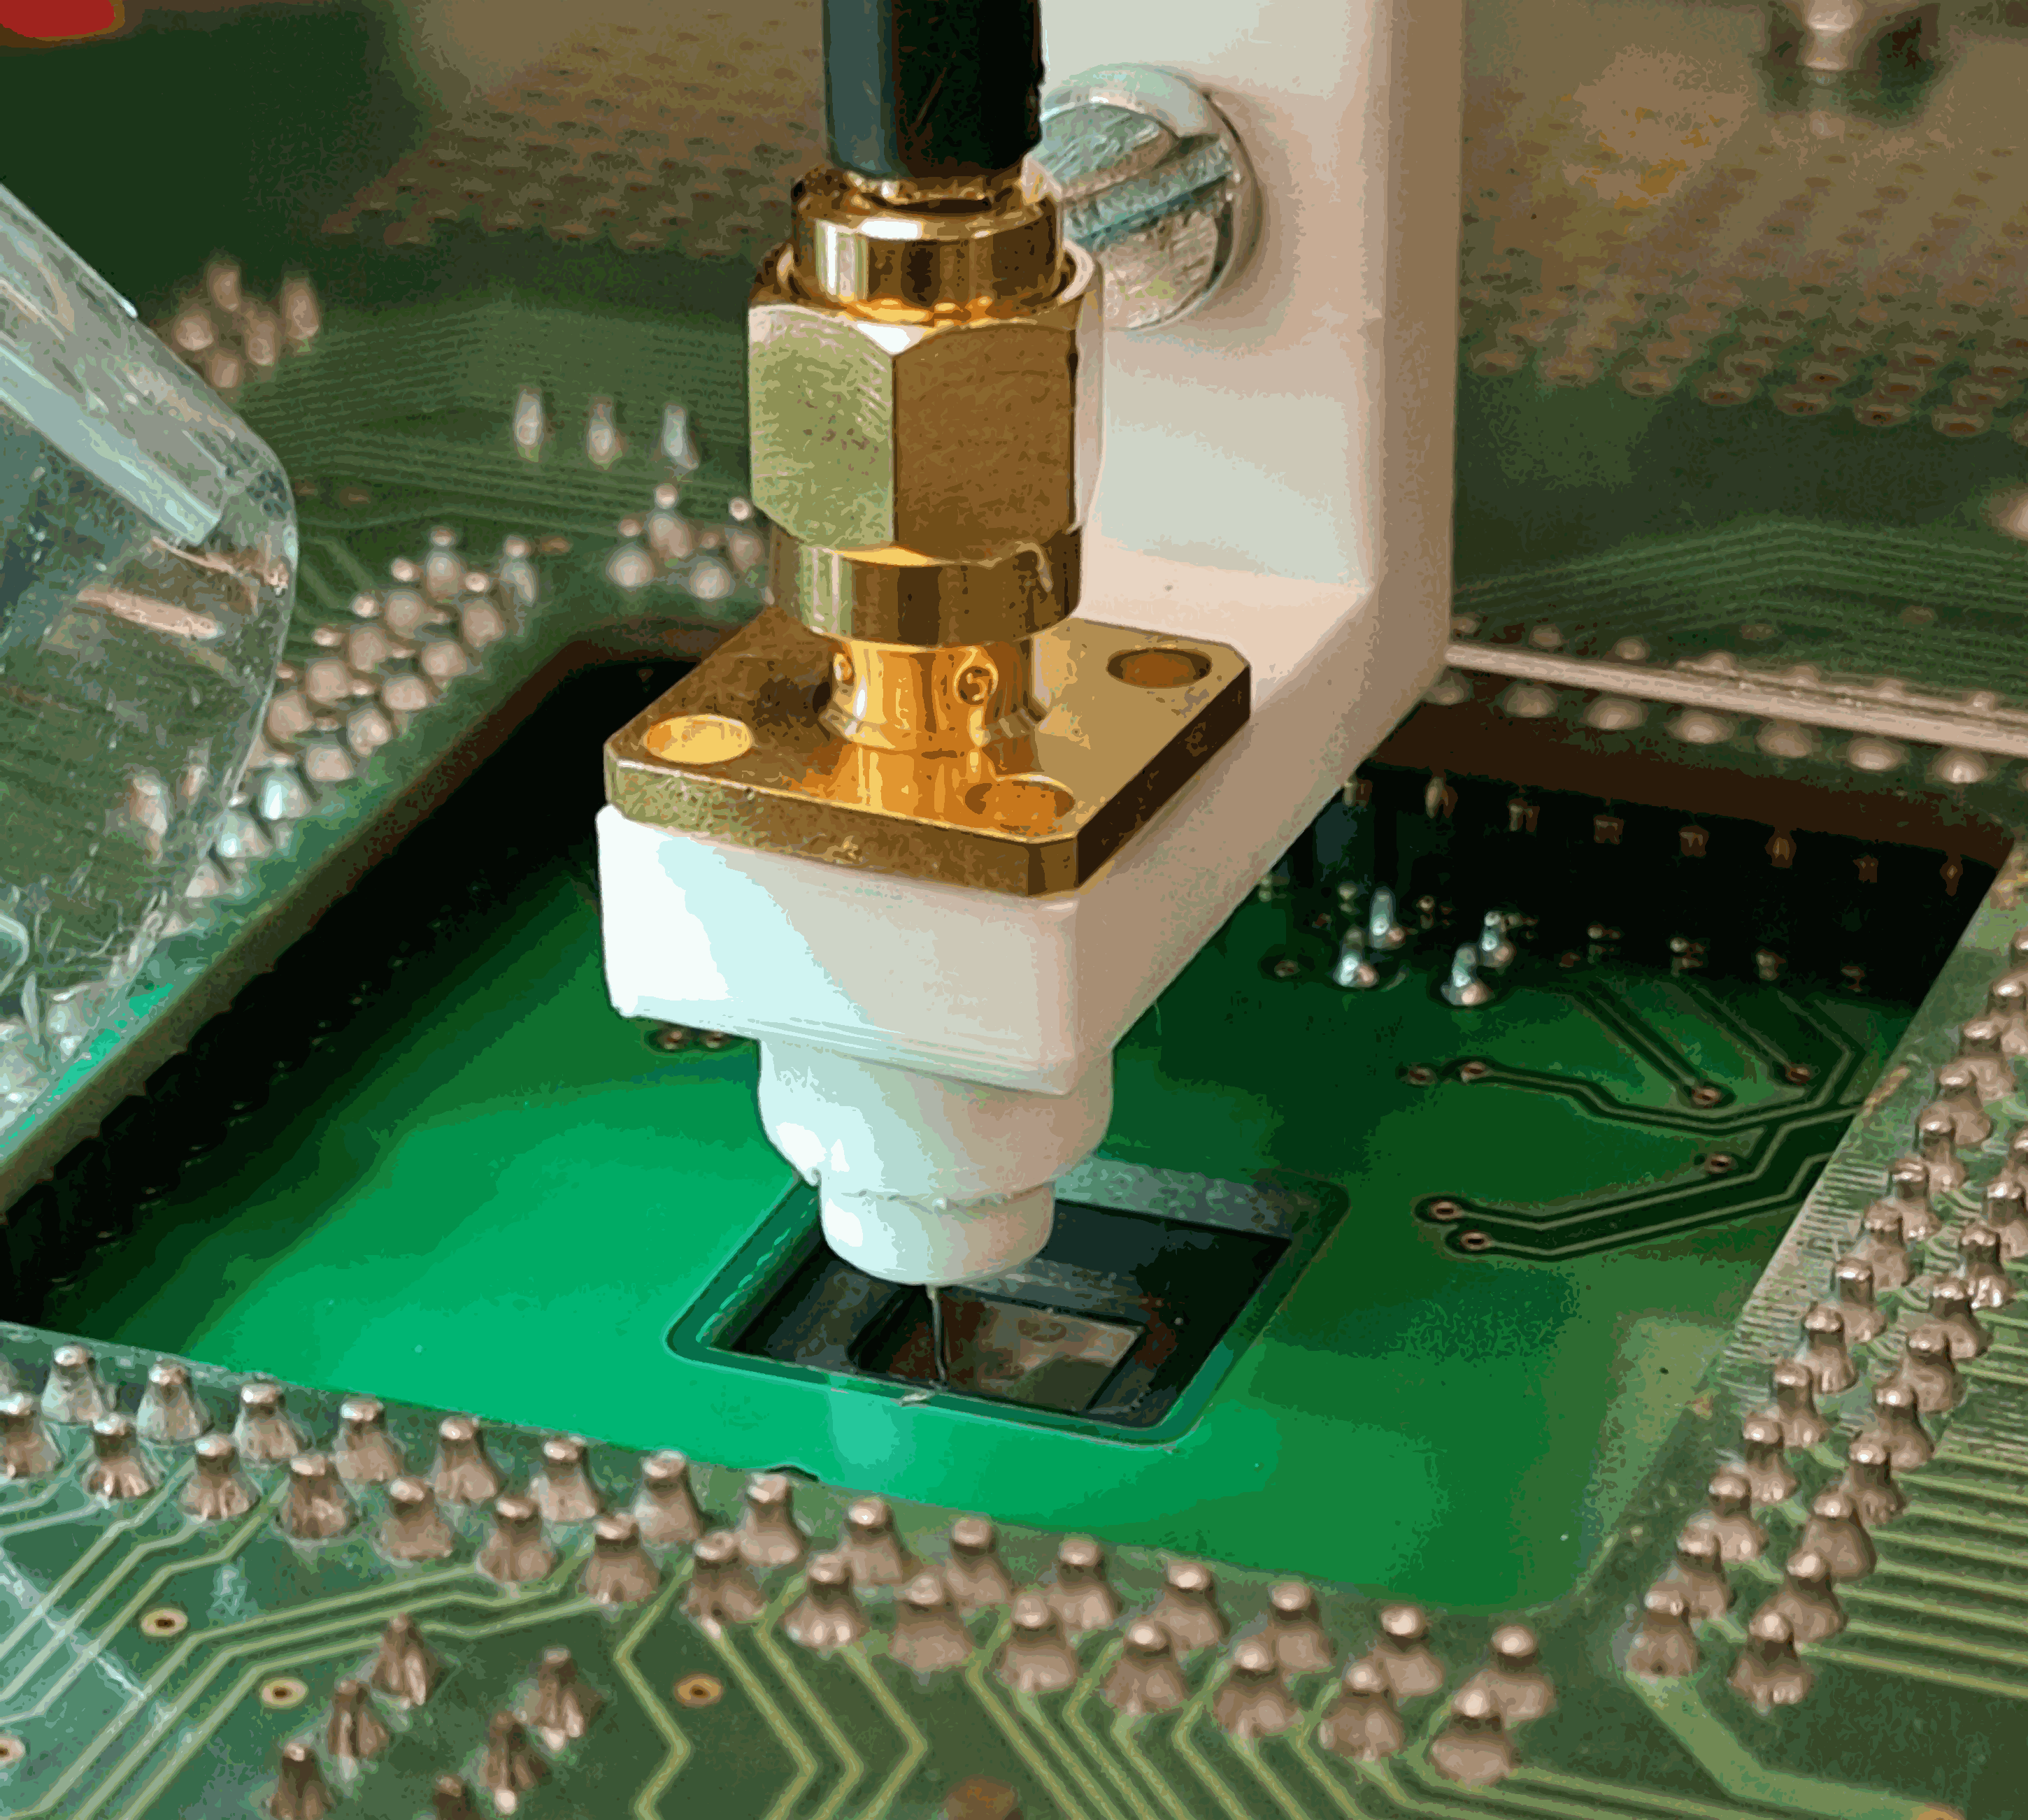
\includegraphics[height=6.8cm]{2_goodPractices/figures/sondeBBI.pdf}
        \caption{BBI metallic probe in mechanical contact with IC target}
        \label{subfig:sondeBBI}
    \end{subfigure}\hfill
    \begin{subfigure}[t]{7.0cm}
        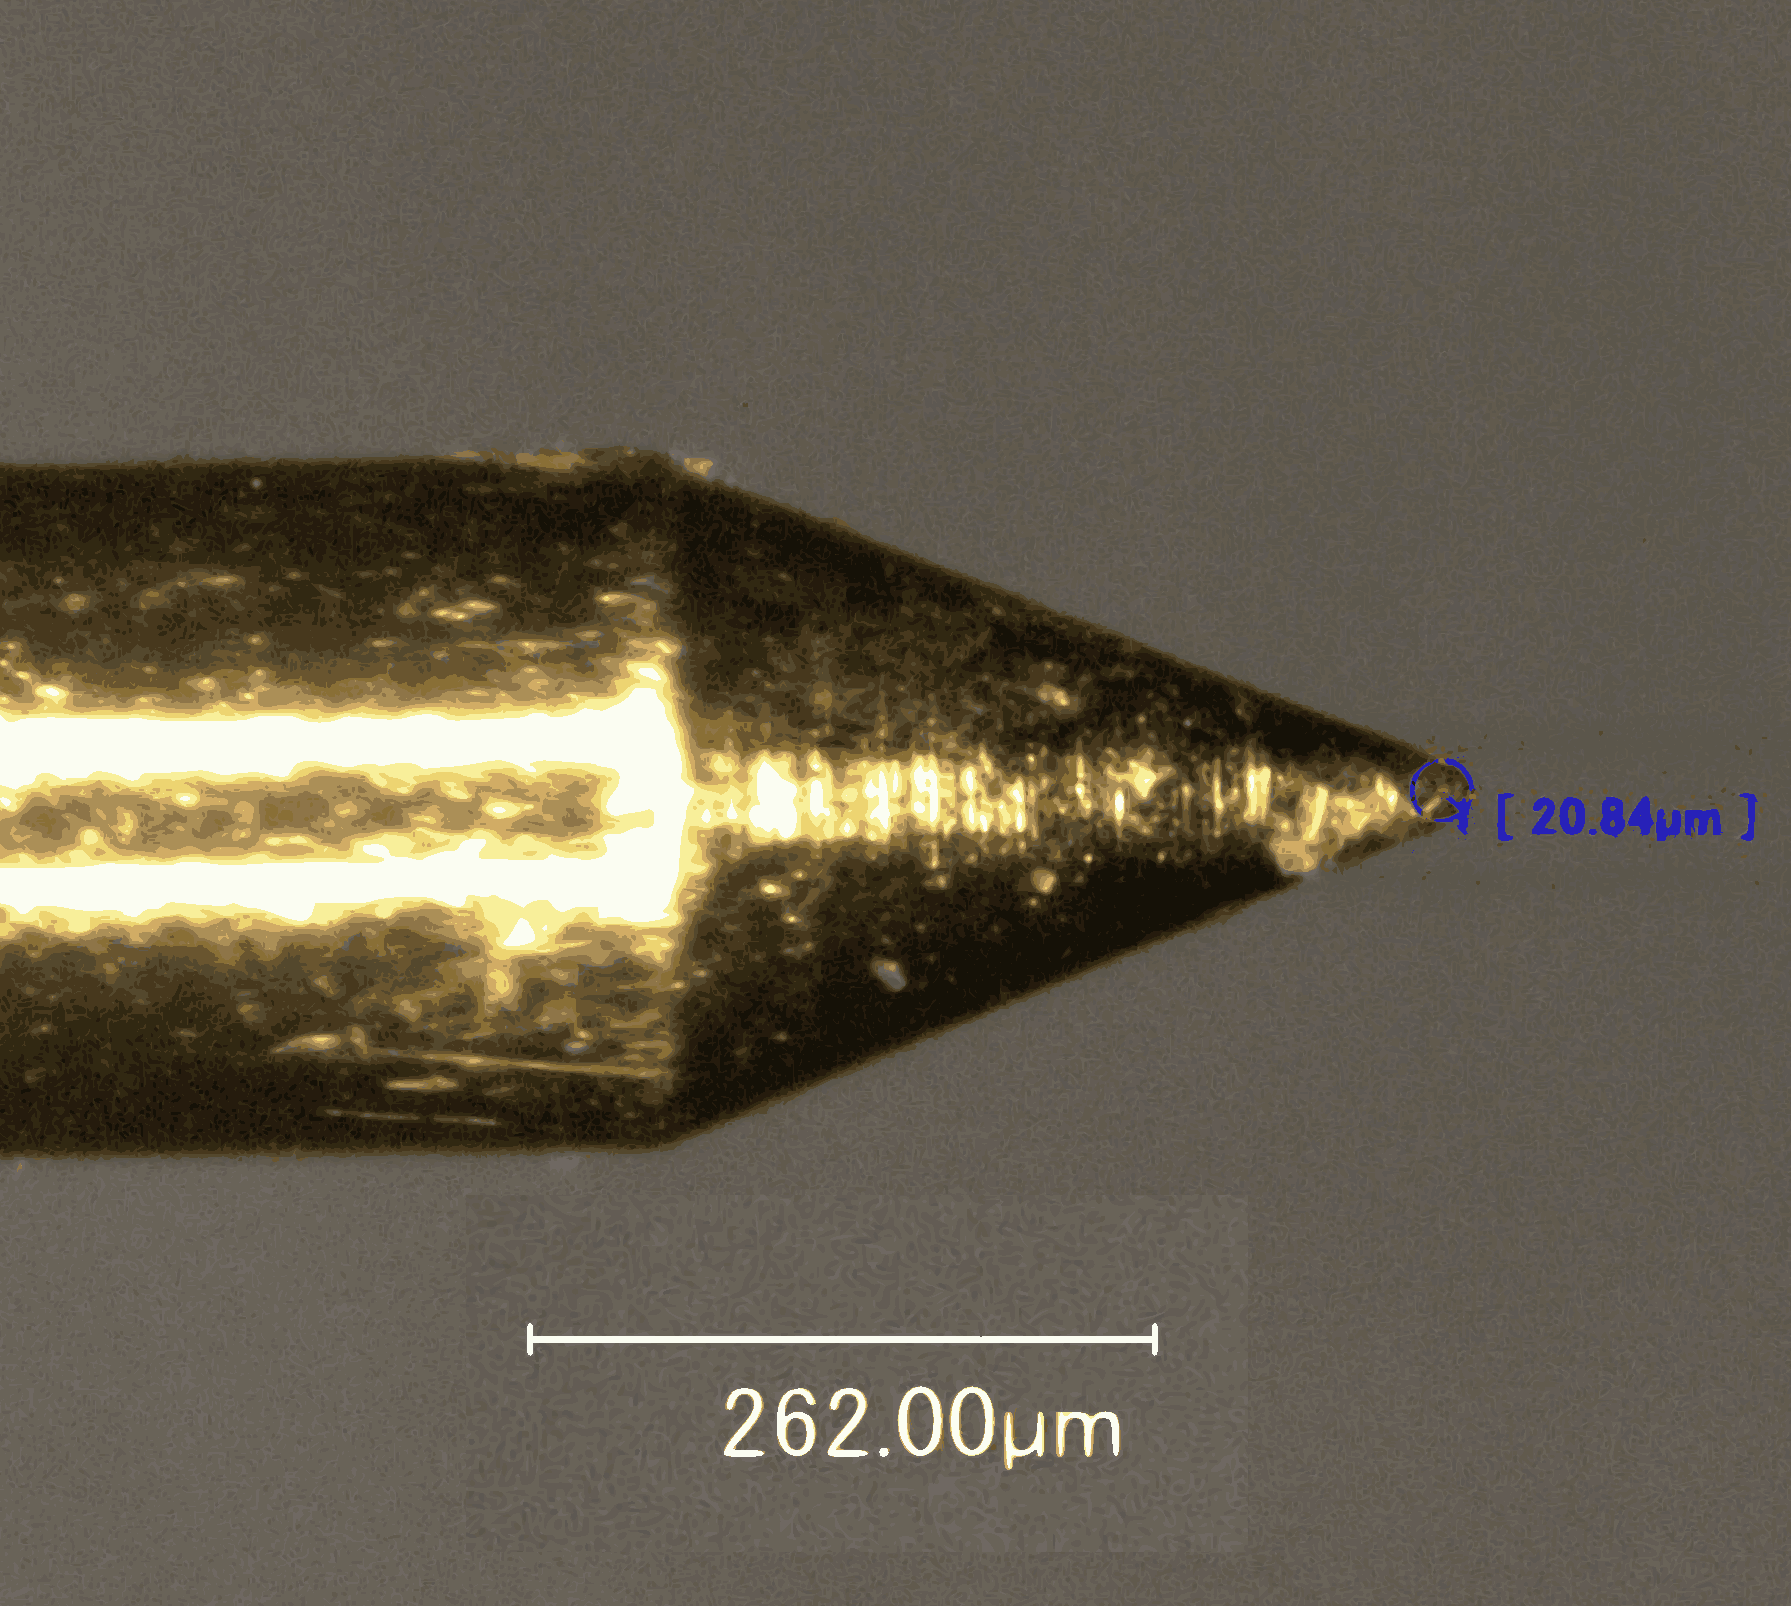
\includegraphics[height=6.8cm]{2_goodPractices/figures/pointeBBI.pdf}
        \caption{BBI metallic probe measurement closer look}
        \label{subfig:pointeBBI}
    \end{subfigure}
    \caption{Dual-well and triple-well inverter silicon sectional view.}
    \label{fig:sondePointeBBI}
\end{figure}
The main piece of equipment when working with BBI is the electrical probe.
It is commonly made with a metal tip, a connector of any sort and a mechanical support to hold everything together.
For the purpose of this work, a custom probe was designed around three simple parts, an SMA connector, in order to have a low-cost, small and standard interconnection, a spring-loaded metallic probe soldered onto the SMA connector, and a custom 3D printed support to hold the structure together.
Fig. \ref{fig:sondePointeBBI} shows detailed pictures of the designed BBI metallic probe, with a global view in operation on Fig.\ref{subfig:sondeBBI}, and a photograph under a microscope of the probe's tip-end on Fig. \ref{subfig:pointeBBI}, allowing to measure its actual size before the first usage.
The metallic probe used has a 0.635 mm diameter and is 16.35 mm long. The specified maximum nominal current of the probe is of 1.5 A, and the electrical contact resistance measures 70 m\textOmega.


\begin{figure}[H]
    \centering
    \includegraphics[width=\textwidth]{2_goodPractices/figures/picoemp-red.jpeg}
    \caption{ChipSHOUTER\textregistered-PicoEMP from NewAE Technology Inc.}
    \label{fig:newAeChipShouter}
\end{figure}
Another fundamental piece of equipment for the practice of BBI is the voltage pulse generator.
It is, generally, the most expensive hardware tool required.
However, nowadays, cheap solutions are easily available, like the NewAE Technology Inc. ChipSHOUTER\textregistered-PicoEMP for example, illustrated in Fig. \ref{fig:newAeChipShouter}.
In addition to being cheaper than most industrial solutions, its design sources are available online, making it a future-proof solution.
In contrast to more expensive solutions, it has inevitably some drawbacks:
\begin{itemize}
    \item The output transformer is low-power, around up to 200 mW
    \item Its recovery time is slow, from 1 to 4 seconds between pulses
    \item It can generate maximum voltage pulses of approximately 250 V
    \item There is no pre-calibration
    \item The pulse width control is not as reliable as other solutions
\end{itemize}


\begin{figure}[H]
    \centering
    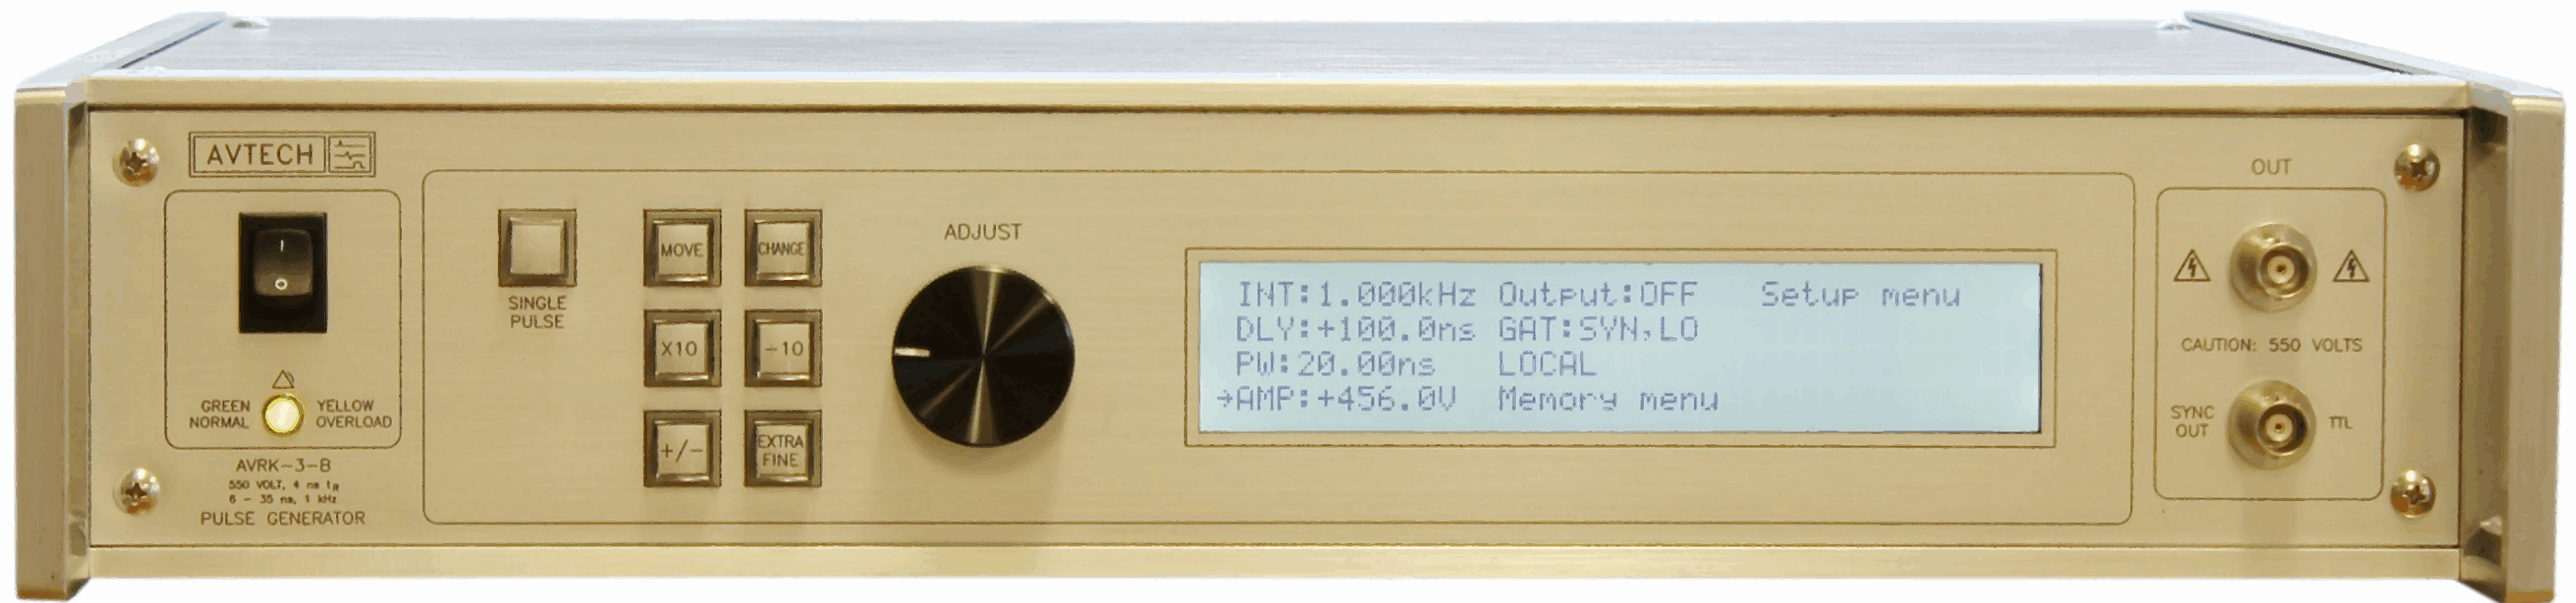
\includegraphics[width=\textwidth]{2_goodPractices/figures/avrk4b.pdf}
    \caption{Front side of the Avtech Electrosystems Ltd. AVRK-4-B High Voltage Pulser}
    \label{fig:avrk4b}
\end{figure}
Nevertheless, for this work, the generator used in all experiments is from the company Avtech Electrosystems Ltd., specifically the model AVRK-4-B, shown in Fig. \ref{fig:avrk4b}.
It is a high-speed and high-voltage generator, specified to work with 50 \textOmega loads.
Its main specifications are the following:
\begin{itemize}
    \item Voltage pulse amplitude from 150 V to 750 V with positive and negative polarities
    \item Pulse width ranging from 6 ns to 20 ns
    \item Rise time (resp. fall-time) for positive (resp. negative) pulses of 4 ns
    \item Up to 1000 pulses per second
    \item GPIB remote control
    \item Propagation delay under 150 ns
    \item DC-coupled output
\end{itemize}

Then, the central piece of equipment of any fault injection method is the IC target.
In our work, the focus was made on an STM32F439VIT6 LQFP100 micro-controller.
It is a moderately modern IC commonly used nowadays.
It was chosen because it embeds a dedicated cryptographic core, able to do DES or AES not to cite them all.
The IC is manufactured with a bulk 90 nm process.
Its core clock frequency goes up to 180 MHz, and it embeds 256 kB of RAM and 2 MB of Flash memory in two separate banks.

\subsection{The software \DDC}
\label{chap2:intro:platEquip:software}
Because several simulations are performed for the purpose of this work, different piece of software are used.
In order to perform every electrical simulations, we used \mbox{Synopsys\textregistered's PrimeSim HSPICE}.
It allows fast simulations with parallel calculation of large netlists.
The computer used for these simulations is made around a 48 cores, 96 threads CPU, alongside 420 GB of usable system memory.
As we will study further in Chapter \ref{chap:3icModeling}, the considered netlists are procedurally generated.
To that end, we developed an algorithm, implemented in Python.
It allows automatic generation of every netlist, minimizing user intervention, therefore drastically reducing errors, especially when considering the size of the simulated netlists.
Indeed, they are not complex in their structure, as they are composed of resistors, capacitors and diodes, but the amount of components ranges from one million for the smallest, to 4.7 millions for the biggest.
The main limitation in simulating these netlists lies in the available system memory, as it is the first bottleneck to appear.
In fact, simulating the smallest ICs takes up to 76 GB of memory during the transient simulation.
As the memory usage scales linearly with the number of components, and because when doubling the width and height, the IC surface quadruples, the same applies for the components count.
Therefore, simulating the biggest ones takes up to 420 GB of system memory, which represents an IC size of 1.1 mm by 1.2 mm.
In addition to the memory consumption, the time required is also an important factor.
Effectively, the smallest ICs take up to four hours and ten minutes with 8 CPU threads (which is close to the maximum HSPICE can do for our netlists).
